\documentclass[a4paper,10pt]{article} \usepackage[utf8]{inputenc}
\usepackage[hidelinks]{hyperref} \def\UrlBreaks{\do\/\do-} % breaks long url in
% references
\usepackage{graphicx} \usepackage[english]{babel} \usepackage{listings}
\usepackage{cite}
\usepackage[labelfont=it,
textfont={it},singlelinecheck=on,justification=centering]{caption}
\usepackage{amsmath} \usepackage{float} \usepackage{xcolor}

\lstset{basicstyle=\ttfamily\footnotesize,breaklines=true} \lstset{numbers=left,
numberstyle=\tiny, stepnumber=1, numbersep=5pt} \lstset{language=TeX}
\setlength{\parskip}{1em} \renewcommand{\baselinestretch}{1.2}
\newcommand{\x}[1]{{\tt #1}} \newcommand{\code}[1]{{\tt #1}}
\newcommand{\todo}[1]{{\color{red} TODO #1 }}


\title{\textbf{Storj\\A Decentralized Cloud Storage Network Framework}}
\author{\\ \parbox{\linewidth}{\centering\small Alex Bender (bender@storj.io),
Alex Leitner (alex@storj.io),\\ Benjamin Sirb (bens@storj.io), Braydon Fuller
(braydon@storj.io),\\ Bryan White (bryan@storj.io), Chris Pollard
(cpollard1001@gmail.com),\\ Dennis Coyle (dennis@storj.io), Dylan Lott
(dylan@storj.io),\\ Garrett Ransom (garrett@storj.io), Gordon Hall
(gordonhall@openmailbox.org),\\ James Hagans (jhagans@storj.io), James Prestwich
(james@storj.io),\\ John Gleeson (jg@storj.io), Josh Brandoff
(josh@brandoff.is), JT Olio (jt@storj.io),\\ Kaloyan Raev (kaloyan@storj.io),
Kishore Aligeti (kishore@storj.io),\\ Nadine Farah (nadine@storj.io), Natalie
Villasana (nat@storj.io),\\ Patrick Gerbes (patrick@storj.io), Philip Hutchins
(philip@storj.io),\\ Shawn Wilkinson (shawn@storj.io), Tome Boshevski
(tome@storj.io)}\\ \\ \small \url{https://github.com/storj/whitepaper} } \date
{June 24, 2018 \\ v3.0}

\begin{document} \maketitle

\begin{abstract} Decentralized cloud storage is attractive for a number of
reasons. Eliminating central control allows users to store and share data
without reliance on a third-party storage provider. Decentralization mitigates
many traditional data failures and outages while simultaneously increasing
security and privacy. At a greater rate than any single entity can afford, it allows
market forces to innovate on cheaper ways to provide storage. While there
are many ways to build such a system, there are some specific responsibilities
any given system should address. Based on our experience with petabyte-scale
storage systems, we introduce a modular framework for considering these
responsibilities and building such a system. Additionally, we describe initial concrete
implementations for each responsibility of the framework. \end{abstract}

\todo{
Remaining big todo items:
\begin{itemize}
\item Datascience: write an appendix about repair bandwidth based on node
  churn and uptime
\item Datascience: Write an appendix about how we select RS numbers
\item Eng/marketing: Quality control/branding section - talk about how we
  plan to ensure heavy client quality by quality control evaluations, formal
  partnerships, relationships, and not letting poor quality heavy clients
  use the brand.
\item Eng: Walkthroughs - highly detailed walkthroughs of how each op works
\begin{itemize}
\item Upload walkthrough
\item Download walkthrough
\item Delete walkthrough
\item List walkthrough
\item Repair walkthrough
\item Payment walkthrough
\item Export/import walkthrough
\end{itemize}
\item Alex/JT: Bandwidth allocation protocol
\end{itemize}

Remaining medium todo items:
\begin{itemize}
\item Anyone: Make sure this paper explains conclusively why we're doing v3 and
  why we won't have to do a v4 - difference between framework vs concrete
  sections
\item Anyone:
  Clean up distributed consensus positioning in the Metadata section.
\item JT: Move merkle-tree-based-filesystem idea to future work section
\item Eng: Describe how path encryption works
\item Eng: Describe payer (heavy client) ids and why they're needed
\item Eng: General data repair framework description
\item Anyone: Clean up attacks section
\item Anyone: Clean up selected calculations section
\item Eng: more macaroon details
\end{itemize}

Remaining little todo items:
\begin{itemize}
\item Anyone: Write the security and privacy requirements section
\item Eng: Write a future work section about eliminating TLS handshakes
\item Anyone: Clean up the pacing for the structured file storage section
\item Eng: Write about how piece ids are generated
\item Eng: Describe pointers
\item Eng: Future work section about reputation sharing
\item Eng: Future work section about finding a better data structure than
 a bloom filter for gc
\end{itemize}
}

\section{Introduction}

Storj is a protocol that creates a distributed network for the reliable storage
of data and facilitates payment for successful data storage and transfer
between peers.
The Storj protocol enables peers on the network to transfer and receive data,
verify the integrity and availability of remote data, and pay other nodes
for storing data.
While not all peers in the network have the same responsibilities,
every peer is an autonomous agent, capable of performing these actions without
significant human interaction.

Many storage products have been created based on distributed storage techniques.
Products such as Wuala, Allmydata, Tahoe-LAFS, Space Monkey, Sia, Maidsafe,
Filecoin, Crashplan, Mozy, HDFS, Storj, S3, GFS, all share one thing in common:
a single computer is not as powerful or as robust as a network. These products
and others attempt to solve a variety of use cases and have many different
requirements, but at a high level, they all operate on the same principles. They
generate redundancy for data in case of failure, store this redundancy in
locations with varying degrees of failure isolation, then keep track of where
the data was placed.

There are a multitude of optimization focuses one could target when creating a
distributed storage system. Speed, capacity, simplicity, trustlessness,
byzantine fault tolerance, security, cost, etc., are all desirable traits in a
storage system. However, independently of anything else, data must be maintained to
prevent data loss, nodes in the system must be able to be communicated with, and
metadata must be kept track of.

We propose a framework that will allow us to choose some reasonable tradeoffs
and then iterate on improvements to components of the system without changing
the overall system.
We accomplish this by breaking the design up into a collection
of relatively independent concerns, and then bring them together to form the
final protocol.

After this first introduction section, the rest of the paper is divided into 4
sections. In Section \ref{sec:design_constraints} we discuss the design space
in which Storj operates in and elaborate on specific design constraints that
focus what we plan to optimize for.
Section \ref{sec:framework} covers our framework and proposes a simple
concrete implementation of each component.
Section \ref{sec:product_details} covers specific details
about how we will deliver this implementation to users. Section
\ref{sec:future_work} covers future areas of research.

\section{Storj design constraints and
considerations}\label{sec:design_constraints}

Before designing a system, it's important to understand its requirements.
We will begin with a discussion of Storj's design constraints.

\subsection{S3 compatibility}

The flagship cloud storage product is Amazon's Simple Storage Service, or S3 for
short. Most cloud storage products provide some form of compatibility with the
S3 API.

Until a decentralized cloud storage protocol is the {\em lingua franca} of
storage protocols, we must create a graceful transition from centralized providers. 
For users with data currently stored on a centralized provider, this will alleviate 
any switching costs.

Our objective is for Storj to compete successfully in the wider cloud storage 
industry and bring decentralized cloud storage to the mainstream -- thus enabling 
more people greater security and less centralized control. To achieve this goal, 
applications built against S3 should be able to be configured to work with Storj with 
minimal friction and changes. Imagine if 90\% of existing application services could switch to Storj with a
single configuration change. \todo{maybe talk about s3 market penetration?} This adds strong requirements on feature set, 
performance, and durability.

\subsection{Device failure and churn}

For any storage system, but especially a distributed storage system, component
failure is a guarantee. All hard drives fail after enough wear
\cite{backblaze-hd-2018-q1}, and the servers providing the network access to
these hard drives will eventually fail, too. Network links die, power is lost,
and storage mediums become unreliable. For data to outlast individual component
failure, data must be stored with enough redundancy to recover from failure.
Perhaps more importantly, no data should be assumed to be stationary and all
data must eventually be moved. In such an environment, redundancy, data
maintanance, repair, and replacement of lost redundancy are facts of life, and
the system must account for these issues.

Decentralized systems are additionally susceptible to high churn rates, where
potential participants join the network and then leave for various reasons, well
before their hardware has actually failed. A network with a high churn rate will
use a large amount of bandwidth just to ensure durability of the data, and such
a network will fail to scale. As a result, a scalable, highly durable storage
system must prefer stable nodes and endeavor to keep the churn rate as low as
possible.

Despite the chance of hardware failure, Maymounkov et al. found that in
decentralized systems, due to churn rates the probability of a node staying on
for an additional hour as a member of the network is an {\em increasing}
function of uptime \cite{kad}. In other words, the longer a node is a
participant in the network, in general the more likely it is to continue
participating. This gives our system a strong incentive to prefer long-lived,
stable nodes.

See Appendix \todo{} for a discussion about how repair bandwidth varies as a
function of node churn and uptime.

\subsection{Latency}

Decentralized, distributed storage has massive opportunities for parallelism
with transfer rates, processing, and a number of other factors. Parallelism by
itself is a great way to increase overall throughput even when individual
network links are slow. However, parallelism cannot by itself improve {\em
latency}. If an individual network link has fixed latency and is a required part
of an operation, the latency of the overall operation will be bound from below
by the latency of the required network link. Therefore, a distributed system
intended for high performance applications must aggressively optimize for low
latency, both at the individual process scale and at the overall architecture
scale.

We emphasize an architectural strategy aimed at achieving low latency by
focusing on eliminating the need to wait for long tails \cite{tail-at-scale}. 
{\color{red}What are long tails?}
The goal is a protocol that allows for every request to be satisfiable by the
fastest nodes participating in any given transaction, without waiting for a slow
subset. Focusing on operations where the result is only dependent on the fastest
nodes turns what could be a potential liability (highly variable performance
from individual actors) into a great source of strength for a distributed
storage network.

\subsection{Bandwidth}

Global bandwidth availability is increasing year over year; however, access to
high-bandwidth internet connections is unevenly distributed. While users in some
countries can easily access symmetric, high-speed, unlimited bandwidth, users in
other countries may have significant difficulty in obtaining access to the same.
In the United States, the way many residential internet service providers provide
internet presents two specific challenges for designers of a
decentralized network protocol. The first challenge is that the internet
connection is often asymmetric. Customers subscribe to internet service
based on an advertised download speed, but the upload speed is potentially an
order of magnitude or two slower. The second challenge is that bandwidth is
sometimes "capped" at a fixed amount of traffic per month. For example, in many
markets, Comcast poses a one terabyte per month bandwidth cap with stiff fines
for customers who go over. Such caps impose
significant limitations on the bandwidth available at any given moment.
An internet connection with a throughput of 10 MB/s and a cap of 1
TB/month may not average more than 385 KB/s over the month without going
over the monthly bandwidth cap.

With device failure and churn guaranteed, any decentralized system will have a
corresponding amount of repair traffic. It is therefore important to make sure
there is enough headroom for the bandwidth required by data maintenance, over
and above that required for data storage and retrieval. Designing a
storage system that is careless with bandwidth usage would be to relegate that
system below storage providers with access to unlimited high-speed bandwidth,
recentralizing the system to some degree. To keep the storage system as
decentralized as possible and for it to work in as many environments as
possible, bandwidth usage must be aggressively minimized.

Please see Appendix \todo{} for a discussion on how available bandwidth,
combined with required repair traffic, limits usable space.

\subsection{Security and privacy}

\todo{we want to make sure users' data privacy is protected}

\subsection{Object size}

Broadly, large storage systems can be classified into two groups by average
object size. When storing lots of small bits of information, generally a
database is the preferred route. On the other hand, when storing lots of large
files, an object store or filesystem is ideal. We classify a "large" file as a 
few megabytes or greater.

The initial product offering by Storj Labs is designed to function primarily as
an object store for larger files. While future improvements may enable
database-like use cases, the predominant use case described by this paper is
object storage. Protocol design decisions are made with the assumption that the
vast majority of objects stored will be a couple of megabytes or more. It is
worth pointing out that this will not negatively impact use cases that require
lots of files smaller than a megabyte. Such cases can admit a packing
strategy, where many small files are aggregated and stored together as one large
file. As the protocol has streaming support, small files can be retrieved
without requiring full retrieval of any aggregated object they were packed into.

\subsection{Byzantine Fault Tolerance}

Unlike datacenter-based solutions like Amazon S3, Storj operates in an untrusted
environment, where individual storage nodes are not necessarily assumed to be
trustworthy. Storj operates over the public internet, and allows anyone to sign
up to become a storage node.

We adopt the BAR (Byzantine, Altruistic, Rational) model \cite{bar} to discuss
participants in the network.
{\em Byzantine} nodes may deviate arbitrarily from the suggested protocol for
any reason. Some examples include nodes that are broken, nodes that are
trying to cheat the suggested protocol to their advantage, or nodes that
are actively trying to sabotage the protocol. In general, a Byzantine node is
one that optimizes for a utility function that is independent of the one
given for the suggested protocol.
Inevitable hardware failure aside, {\em Altruistic} nodes
participate in a proposed protocol even if the rational choice is to deviate.
{\em Rational} nodes participate exactly when it is in their net benefit to do
so, and may depart for the same reason.

Some distributed storage systems (e.g., Amazon S3) operate in an environment
where all nodes are altruistic {\color{red}add citation?}.
Storj operates in an environment where a
majority of storage nodes are rational and a minority are byzantine. Storj
assumes no altruistic nodes. Any
potential design must account for this distinction.

\section{Framework and concrete implementation}\label{sec:framework}

At a high level, there are three major operations in the system: storing data,
retrieving data, and maintaining data.

\begin{description}

\item[Storing data] When data is stored with the network, the client encrypts
it and breaks it up into multiple little pieces. It then distributes the pieces to peers in
the network then generates and stores some metadata about where to find the data
again.

\item[Retrieving data] When data is retrieved from the network, 
it first recovers the metadata about where to find the pieces. 
Then the pieces are retrieved and the original data is reconstructed 
on the client's local machine.

\item[Maintaining data] Data is maintained in the network with nodes replacing
missing pieces when the amount of redundancy drops below a certain threshold.
The data is reconstructed and the missing pieces are regenerated and replaced.

\end{description}

To make this system feasible while satisfying our design constraints, we will
need to solve a number of complex challenges. Inspired by Raft \cite{raft}, we
break up the design into a collection of relatively independent concerns and
then combine them to form the desired protocol. One important benefit is it makes 
updating individual components much easier without having to rearchitect the rest 
of the network. The individual components are:

\begin{enumerate}
\item Storage nodes
\item Peer-to-peer communication
\item Overlay network
\item Redundancy
\item Structured file storage
\item Metadata
\item Encryption
\item Authorization
\item Audits
\item Data repair
\item Storage node reputation
\item Payments
\item Payer reputation
\item Garbage collection
\end{enumerate}

\subsection{Storage nodes}

The most basic building block is the storage node. The storage node stores and
returns data provided to it. Nodes should provide reliable storage space,
network bandwidth, and appropriate responsiveness. In return, nodes are rewarded
for their participation. Storage nodes will be selected based on a number of
different criteria. Ping time, latency, throughput, disk space, geographic
location, legal restrictions, etc., are all important factors that may need to
be considered. This means that node selection almost certainly must be an
explicit process.

\subsubsection{Concrete implementation}

Storage nodes will support three methods: \code{get}, \code{put}, and
\code{delete}. Storage nodes store {\em pieces} (to be described in more detail
later). Each method will take a {\em piece ID}, a {\em payer ID} and signature
by the payer, an optional TTL, and the other metadata required by the bandwidth
allocation protocol (also to be described later).

The \code{put} operation will take a stream of bytes and store the bytes such
that any subrange of bytes can be retrieved again via a \code{get} operation.
\code{get} operations are expected to work until the TTL expires (if a TTL was
provided), or until a \code{delete} operation is received, whichever comes
first.

The {\em payer ID} forms a namespace. An identical {\em piece ID} with a
different {\em payer ID} refers to a different {\em piece}.

Storage nodes should allow administrators to configure maximum allowed disk
space usage and maximum allowed bandwidth usage over the last rolling 30 days.
Storage nodes should keep track of how much is remaining of both. Storage nodes
should reject operations that do not have a valid signature from the appropriate
payer.

\subsection{Peer-to-peer communication}

All peers on the network will need to communicate. The framework requires a
reliable and ubiquitous protocol that all peers speak that:

\begin{itemize}
\item provides peer reachability, even in the face of firewalls
and NATs. This may require techniques like STUN, relays, etc.
\item provides authentication, where each participant knows
exactly the identity of the peer with whom they are speaking.
\item provides privacy, where only the two peers
know what transfers between them.
\end{itemize}

\subsubsection{Concrete implementation}

Initially, we'll be using gRPC \cite{grpc} on top of TLS on top of $\mu$TP
\cite{utp} with added STUN functionality. Over time, we'll be replacing TLS to
reduce round trips due to connection handshakes in situations where the data is
already encrypted and forward secrecy isn't necessary. \todo{} See the Future
Work section for more details. Gateways will be provided that allow for more
standard protocols such as HTTPS.

As in S/Kademlia \cite{skad}, the {\em node ID} will be the hash of a public key
and will serve as a proof of work for joining the network. Unlike Bitcoin proof
of work \cite{bitcoin}, the work will be dependent on how many {\em trailing}
zero bits one can find in the hash output. This means that the node ID will
still be usable in a balanced Kademlia \cite{kad} tree.

Each node will operate its own certificate authority, which requires a
public/private keypair and a self-signed certificate. The certificate authority
should ordinarily be kept in cold storage to prevent key loss.

Each node will also have revokable leaf key pair and certificate, signed by
the node's certificate authority. Nodes will use this leaf keypair for actual
communication. Should the leaf become compromised, the node can issue a new
leaf and a new entry in a certificate revocation list.

The {\em node ID} will be determined from the certificate authority
by hashing the DER-encoded public key.

\begin{equation}
\text{NodeID} = \text{SHA256}(\text{Pu})
\end{equation}

It's important that the certificate authority private key be managed with good
operational security as key rotation for the certificate authority will require
a brand new node ID.

When using TLS, every peer can ascertain the ID of the node with which it is
speaking by validating the certificate chain and hashing its peer's
certificate authority's public key. It can then be estimated how much work went
into constructing the node ID by considering the number of 0 bits at the end of
the ID.

For the few cases where a node cannot achieve a successful hole punch through a
NAT or firewall via STUN, uPnP, NATPmP, or a similar technique, manual
intervention and port forwarding will be required.

\subsection{Overlay network}

If, given a peer's network address, any other peer can connect to it, the
framework requires a system to look up peer network addresses by node ID in the
first place. An {\em overlay network} can be built on top of our peer-to-peer
communication component that provides functionality similar to DNS, where a
node's ID can be resolved to an ephemeral network address for communication.

\subsubsection{Concrete implementation}

The Kademlia DHT serves as a key-value store with a built-in node lookup
protocol. We utilize this protocol to achieve DNS-like functionality for node
lookup, while ignoring the storage aspects of the Kademlia protocol due to some
issues around value republishing, limits to network growth rate, and so on.
However, using a DHT will make it difficult to achieve millisecond-level
response times when multiple DHT lookups must happen for every operation, so
more work is necessary to achieve our performance goals. Fortunately, caching
address information for an entire network of 80k nodes (for example) can be done
with 3MB of memory, so the DHT can be sped up with some simple, optional
caching.

Because a cache of the DHT can be untrusted (and peer-to-peer communication is
authenticated to avoid man-in-the-middle-attacks anyway), some well-known
community-run DHT caches can be provided that simply attempt to talk to every
storage node every so often, such as every hour, evicting nodes from their
cache that have not been seen recently.
Since nodes are expected to be long lived with good uptime, they
are expected to have stable addresses that don't change often on the order of
more than once an hour. Thus, such a cache will add a massive performance boost, even when slightly stale.
In addition, the protocol will be resilient against an expected degree of node
churn, so having a small number of stale addresses in a DHT cache will not alter
the expected performance of the network. Furthermore, we avoid a number of known
attacks by using the S/Kademlia extensions. \cite{skad}

\todo{talk about how we're using kademlia to advertise disk space and bandwidth
availability, and then storing that information in the cache}

\subsection{Redundancy}

At any moment, any storage node could go offline permanently. Our redundancy
strategy must store data in a way that provides access to the data with high
probability, even though any given number of individual nodes may be offline. To
achieve a certain level of {\em durability} (the probability that data will
remain available in the face of failures), many products in this space use
simple replication. Unfortunately, this ties durability to the network {\em
expansion factor}, which is the storage overhead for reliably storing data.

As an example, suppose a certain desired level of durability requires a
replication strategy that makes eight copies of the data. This yields an
expansion factor of 8x, or 800\%. This data then needs to be stored on the
network, using bandwidth in the process. Thus, more replication results in more
bandwidth usage for a fixed amount of data. As discussed in the protocol design
constraints, high bandwidth usage prevents scaling, so this is an undesireable
strategy for ensuring a high degree of file durability. Instead, {\em erasure
codes} are a more general and more flexible scheme for manipulating data
durability without tying it to bandwidth usage. Importantly, erasure codes allow
changes in durability without changes in expansion factor!

An erasure code is often described by two numbers, $k$ and $n$. If a block of
data is encoded with a $(k,n)$ erasure code, there are $n$ total generated {\em
erasure shares}, where only any $k$ of them are required to recover the original
block of data. If a block of data is $s$ bytes, each of the $n$ erasure shares
is roughly $s/k$ bytes. Besides the case when $k=1$ (replication), all erasure
shares are unique. Interestingly, the durability of a $(k=20,n=40)$ erasure code
is better than a $(k=10,n=20)$ erasure code, even though the expansion factor
(2x) is the same for both! Intuitively, this is because the risk is spread
across more nodes in the $(k=20,n=40)$ case. These considerations make erasure
codes an important part of our general framework.

With the simplifying assumption that every node has an equal probability of
failure $p$, one can gain more intuition by modeling file durability as the CDF
of the binomial distribution, as seen in Equation \eqref{eq:binom_cdf}. In this
case, $P(D)$ represents the probability that at most $n-k$ erasure shares are
lost for a given file, so that $n-(n-k)=k$ erasure shares of the file remain;
i.e. the file can still be rebuilt. The CDF of the binomial distribution is
given by:

\begin{equation} P(D) = \sum_{i=0}^{n-k} \binom{n}{i} p^i
(1-p)^{n-i}\label{eq:binom_cdf}
\end{equation}

\begin{table}[b]
\centering
\begin{tabular}{c c c l}
$k$ & $n$ & Exp. factor & P(D) \\
\hline 2 & 4 & 2 & 99.629999999999996341\%\\
4 & 8 & 2 & 99.956834999999999436\%\\
8 & 16 & 2 & 99.999407567699549748\%\\
16 & 32 & 2 & 99.999999871786737771\%\\
32 & 64 & 2 & 99.999999999999988898\%\\
\end{tabular}
\caption{$P(D)$ for various choices of $k$ and $n$, assuming $p=0.9$.}
\end{table}

\begin{figure} \centering
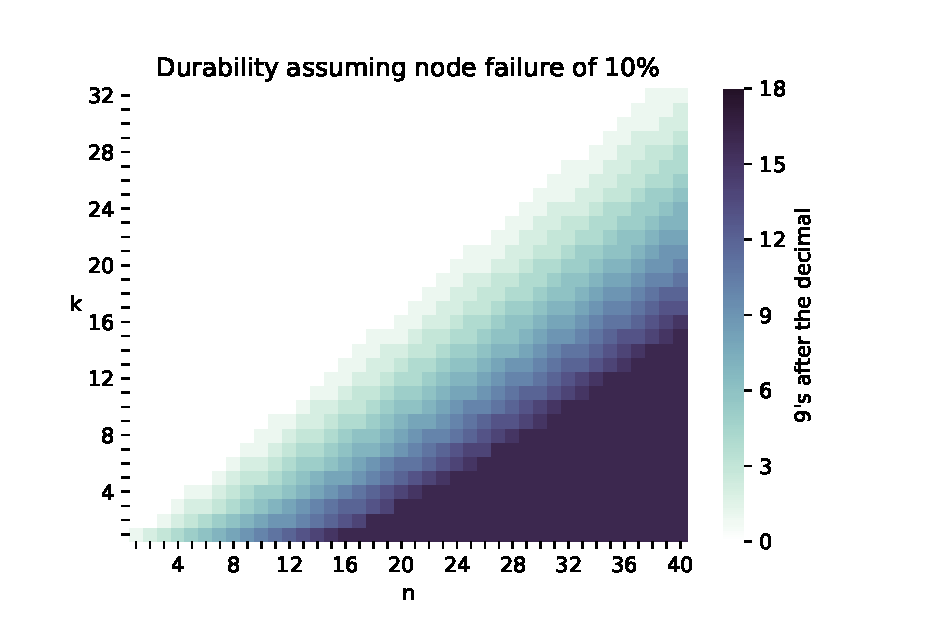
\includegraphics[width=\linewidth]{durability/durability.eps}\label{fig:durability}
\end{figure}

By being able to tweak the durability independently of the expansion factor,
very high durabilities can be achieved with surprisingly low expansion factors.
Because of how limited bandwidth is as a resource, eliminating replication as a
strategy entirely and using erasure codes only for redundancy causes a drastic
decrease in bandwidth footprint and a drastic increase in the funds available
per byte on storage nodes.

\subsubsection{Streaming}

Erasure codes are used in many streaming contexts such as audio CDs and
satellite communications, so it's important to point out that using erasure
coding in general does not make our streaming design requirement more
challenging. Whatever erasure code is chosen for our framework, streaming can be
added on top by encoding small portions at a time, instead of attempting to
encode a file all at once. See the structured file storage section for more
details.

\subsubsection{Long tails}

Erasure codes enable an enormous performance benefit, which is the ability to
avoid waiting for long-tail response times \cite{tail-at-scale}. For uploads, a
file can be encoded to a higher $(k, n)$ ratio than necessary for durability
guarantees. During an upload, after enough pieces have uploaded to gain required
redundancy, the remaining additional uploads can be canceled, allowing the
upload to be blocked by the fastest nodes in a set, instead of waiting for the
slowest nodes. Downloads are similarly improved. Since more redundancy exists
than is needed, downloads can be served from the fastest peers, eliminating a
wait for temporarily slow or offline peers.

\subsubsection{Concrete implementation}

We use the Reed-Solomon erasure code \cite{rs}. For each object that we store
we choose 4 numbers, $k$, $m$, $o$, and $n$, such that $k\le m\le o\le n$.
$k$ and $n$ are the standard Reed Solomon numbers, where $k$ is the minimum
required number of pieces for reconstruction, and $n$ is the total number of
pieces generated during creation.

$m$ and $o$ are the {\em minimum safe} and {\em optimal} values, respectively.
$m$ is chosen such that if the amount of available pieces falls below $m$, a
repair is triggered immediately in an attempt to make sure we always maintain
$k$ or more pieces. $o$ is chosen such that during uploads, as soon as $o$
pieces have finished uploading, remaining pieces up to $n$ are canceled as
described above. $o$ is chosen such that storing $o$ pieces is all that is
needed to achieve the desired durability goals; $n$ is thus chosen such that
storing $n$ pieces would be excess durability.

Our durability story does not end with our selection of these numbers.
Please see section \ref{sec:data_repair} for a discussion about how we repair
data as its durability drops over time.

See \todo{data science: Appendix} for how we select our Reed-Solomon numbers.

\subsection{Structured file storage}

Our design constraints include S3 compatibility. This means we should support
hierarchical objects (paths with prefixes), object metadata, arbitrarily large
files, arbitrarily large amounts of files, and so on. Similarly, our design
constraints require security, so any such metadata must be encrypted.

Provided we have an efficient way to store data, we can build many of these
features on top by means of an {\em injective embedding} (here used in the
mathematical sense). In other words, adding this functionality can be done by
building on top of the basic components we have already created without loss of
generality.

Because so much here depends on concrete
implementation details, our framework is loose in specificity, while our
concrete implementation has significant detail.

\subsubsection{Concrete implementation}

\todo{an introduction before diving into a list of definitions}

\begin{description}
\item[Bucket] A \x{bucket} is an unbounded but named
collection of \x{file}s identified by \x{path}s. Each \x{path} represents one
\x{file}, and every \x{file} has a unique \x{path}.

\item[Path] A \x{path} is a unique identifier for a \x{file} within a
\x{bucket}. A \x{path} is a string of UTF8 codepoints that begins with a forward
slash and ends with something besides a forward slash. More than one forward
slash (referred to as the \x{path separator}) separate \x{path components}.

An example path might be \code{/etc/hosts}, where the \x{path components} are
\code{etc} and \code{hosts}.

We encrypt \x{paths} before they ever leave the customer's application's
computer.

\item[File] A \x{file} is a collection of \x{stream}s. Every \x{file} has
exactly one default \x{stream} and may have 0 or more named \x{stream}s.
Multiple \x{stream}s allow flexible support of extended attributes, alternate
data streams, resource forks, and other slightly more esoteric filesystem
features.

Like \x{path}s, the data contained in a \x{file} is encrypted before it ever
leaves the client computer.

\item[Stream] A \x{stream} is an ordered collection of 0 or more \x{segment}s.
\x{segment}s have a fixed maximum size, and so the more bytes the \x{stream}
represents through \x{segment}s, the more \x{segment}s there are.

\item[Segment] A \x{segment} represents a single array of bytes, between 0 and a
user-configurable maximum \x{segment} size. Breaking large \x{file}s into
multiple \x{segment}s provides a number of security and scalability advantages.

\item[Inline Segment] An \x{inline segment} is a \x{segment} that is small
enough it makes sense to store it "inline" with the metadata that keeps track of
it, such as a \x{pointer}.

\item[Remote Segment] A \x{remote segment} is a larger \x{segment} that will be
encoded and distributed across the network. A \x{remote segment} is larger than
the metadata required to keep track of its book keeping.

\item[Stripe] A \x{stripe} is a further subdivision of a \x{segment}. A
\x{stripe} is a fixed amount of bytes that is used as an encryption and erasure
encoding boundary size. Erasure encoding happen on \x{stripe}s individually,
whereas encryption may happen on a small multiple of stripes at a time. All
\x{segments} are encrypted, but only \x{remote segments} are erasure encoded.

\item[Erasure Share] When a \x{segment} is a \x{remote segment}, its \x{stripe}s
will get erasure encoded. When a \x{stripe} is erasure encoded, it generates
multiple pieces called \x{erasure share}s. Only a subset of the \x{erasure
share}s are needed to recover the original \x{stripe}, but each \x{erasure
share} has an index identifying which \x{erasure share} it is (e.g., the first,
the second, etc.).

\item[Piece] When a \x{remote segment}'s \x{stripe}s are erasure encoded into
\x{erasure share}s, the \x{erasure share}s for that \x{remote segment} with the
same index are concatenated together, and that concatenated group of \x{erasure
share}s is called a \x{piece}. If there are $n$ \x{erasure share}s after erasure
encoding a \x{stripe}, there are $n$ \x{piece}s after processing a \x{remote
segment}. The $i$th \x{piece} is the concatenation of all of the $i$th
\x{erasure shares} from that \x{segment}'s \x{stripe}s.

\item[Piece Storage Node] A node in the network that is responsible for storing
\x{piece}s. These are operated by \x{farmer}s.

\item[Farmer] A person or group that is responsible for running and maintaining
\x{piece storage nodes}.

\item[Pointer] A \x{pointer} is a data structure that keeps track of which
\x{piece storage nodes} a \x{remote segment} was stored on, or the \x{inline
segment} data directly if applicable.

\end{description}

\subsubsection{Files as Streams}

Many applications benefit from being able to keep metadata alongside files. For
example, NTFS supports "alternate data streams" for each file, HFS supports
resource forks, EXT4 supports "extended attributes," and more importantly for
our purposes, AWS S3 supports "object metadata" \cite{s3-object-meta}. Being
able to support arbitrarily named sets of keys/values dramatically improves
compatibility with other storage platforms. Every \x{file} will have at least
one
\x{stream} (the default \x{stream}) and many files may never have another
\x{stream}.

\subsubsection{Streams as Segments}

Because \x{stream}s are used for data (the default \x{stream}) and metadata
(extended attributes, etc.), \x{stream}s should be designed both for small data
and large data. If a \x{stream} only has very little data, it will have one
small \x{segment}. If that \x{segment} is smaller than the metadata it would
require to be stored on the network, the \x{segment} will be an \x{inline
segment} and the data will be stored directly inline with the metadata.

For larger \x{stream}s past a certain size, the data will be broken into
multiple large \x{remote segment}s. Segmenting in this manner has a number of
advantages to security, privacy, performance, and availability.

Maximum \x{segment} size is a configurable parameter. To preserve privacy, it is
recommended that \x{segment} sizes be standardized as a byte multiple, such as 8
or 32 MB. Smaller \x{segment}s may be padded with zeroes or random data.
Standardized sizes help frustrate attempts to determine the content of a given
\x{segment} and can help obscure the flow of data through the network.

Segmenting large files like video content and distributing the \x{segment}s
across the network separately reduces the impact of content delivery on any
given node. Bandwidth demands are distributed more evenly across the network. In
addition, the end-user can take advantage of parallel transfer, similar to
BitTorrent or other peer-to-peer networks.

\subsubsection{Segments as Stripes}

In many situations it's important to be able to access just a portion of some
data. Some large file formats such as large video files, disk images, or file
archives support the concept of seeking, where only a partial subset of the data
is needed for correct operation. In these cases it's useful to be able to decode
and decrypt only parts of a file.

A \x{stripe} is no more than a couple of kilobytes, and encoding a single
\x{stripe} at a time allows us to read portions of a large \x{segment}
without retrieving the entire \x{segment}, allows us to stream data into the
network without staging it beforehand, and enables a number of other useful
features.

Depending on the sizes, \x{stripes} are either encrypted individually or in
small batches. Only a few stripes should be needed for successful
decryption. In either case, \x{stripes} should be encrypted client-side before
being erasure encoded. The reference implementation uses AES256-GCM by default,
but XSalsa20+Poly1305 is also provided. This protects the
content of the data from the \x{farmer} housing the data. The data owner
retains complete control over the encryption key, and thus over access to the
data.

It's important to use authenticated encryption to defend against data corruption
(willful or negligent) with a monotonically increasing nonce to defeat
reordering attacks. The nonce should be monotonically increasing throughout
the entire \x{stream}. If \x{stripe} batch $i$ is encrypted
with nonce $j$, stripe batch $i+1$ should be encrypted with nonce $j+1$. Each
\x{segment} should get a new encryption key whenever the content in the
\x{segment} changes to avoid nonce reuse. \todo{jt: fix this}

\subsubsection{Stripes as Erasure Shares}

Erasure encoding gives us the chance to control network durability in the face
of unreliable \x{piece storage node}s. Erasure encoding schemes often are
described as $(k, n)$ schemes, where $k$ \x{erasure shares} are needed for
reconstruction out of $n$ total. For every \x{stripe}, $n$ \x{erasure share}s
are generated, where the network has an expansion factor of $\frac{n}{k}$.

For example, let's say a \x{stripe} is broken into 40 \x{erasure share}s
($n=40$), where any 20 ($k=20$) are needed to reconstruct the \x{stripe}. Each
of the 40 \x{erasure share}s will be $\frac{1}{20}$th the size of the original
\x{stripe}. All $n$ \x{erasure share}s have a well defined index associated
with them. The $i$th share will always be the same, given the same input
parameters.

Because peers generally rely on separate hardware and infrastructure, data
failure is not correlated. This implies that erasure codes are an extremely
effective method of securing availability. Availability is proportional to the
number of nodes storing the data.

See section \todo{} for a breakdown of how varying the erasure code parameters
affects availability and redundancy.

\subsubsection{Erasure Shares as Pieces}

Because \x{stripe}s are already small, \x{erasure share}s are often much
smaller, and the metadata to keep track of all of them separately would be
immense relative to their size. Instead of keeping track of all of the shares
separately, we pack all of the \x{erasure share}s together into a few
\x{piece}s. In a $(k, n)$ scheme, there are $n$ \x{piece}s, where each
\x{piece} $i$ is the ordered concatenation of all of the \x{erasure share}s with
index $i$. As a result, where each \x{erasure share} is $\frac{1}{k}$th of a
\x{stripe}, each \x{piece} is $\frac{1}{k}$th of a \x{segment}, and only $k$
\x{piece}s are needed to recover the full \x{segment}.

\todo{piece ids are generated as the hmac of a root piece id and the storing
node id}

\subsubsection{Pointers}

\todo{}

\subsection{Metadata}

In the previous section, we discussed how we will break up files, encode them
for redundancy, and then store them in the network. Independently of the
concrete organization and structure of this scheme, there are two types of
metadata that are important to store somewhere for recovery: paths and what
storage nodes received pieces (pointers).

Our framework requires a relatively performant system that can store pointers by
path in a way that supports ordered iteration over those paths. Every time an
object is added, edited, or removed, one or more entries in this metadata
storage system will need to be adjusted. As a result, there could be heavy churn
in this metadata system, and across the entire userbase the metadata itself
could end up being a sizeable amount of data.

To talk more about the scope and scale we expect with some examples, suppose in
a few years this system stores 1 total exabyte of data, where the average object
size is 50MB and our erasure code is such that $n=40$. Each object will use just
one segment, and thus have one pointer each. The pointer will contain
information about the segment encoding, including what $n$ nodes the segment
pieces are stored on. 1 exabyte of 50MB objects is 20 billion objects. If
each pointer is roughly 40*64+192 bytes (info for each node plus the path and
some general overhead), there are over 55 terabytes of metadata to keep track of
(which is still 18,181 times less data to keep track of than an exabyte).
Fortunately, this metadata can be heavily partitioned by user. A user storing a
100 terabytes of 50MB objects will only incur an overhead of 5.5 gigabytes, once
again 18,181 times less data. It's worth pointing out that these numbers vary
heavily with average object size (the larger the object size, the less the
metadata overhead).

One of our framework's primary focuses is making sure this component -- metadata
storage -- is interchangeable per user. Specifically, we expect to ship with
multiple implementations of metadata storage that we will allow users to choose
between. Other systems have spent an enormous amount of time attempting to solve
this problem. We've concluded that multiple {\em good enough} solutions already
exist, and propose using them.

Aside from scale requirements, the desired API is straightforward and
simple: Put (store a pointer given a path), Get (retrieve a pointer given a
path), List (paginated, ordered listing of existing paths), and Delete (remove a
path).

\subsubsection{Aside about distributed consensus}

A long and challenging area of research has been directed toward getting a
group of computers to agree on a set of values, with the goal of constructing a
horizontally-scalable database that works in the face of expected failures
(crash failures, for example: failures where a server simply shuts down).
Fortunately, this research has led to some really exciting technology.

The biggest issue with getting a group of computers to agree is that messages
can be lost. How this impacts decision making is succinctly described by the
"Two Generals' Problem" \cite{two-generals} (earlier described as a problem
between groups of gangsters \cite{two-gangsters}), in which two armies try to
communicate in the face of potentially lost messages. Both armies have already
agreed to attack a shared enemy, but have yet to decide on a time. Both armies
must attack at the same time or else failure is assured. Both armies can send
messengers, but the messengers are often captured by the enemy. Both armies must
know what time to attack and that the other army has also agreed to this time.

Ultimately, a solution to the two generals' problem with a finite number of
messages has been proven to be impossible, so engineering approaches have had
to brace uncertainty by necessity. Many distributed systems make trade-offs to
deal with this uncertainty. Some systems embrace {\em consistency}, which means
that the system will choose downtime over inconsistent answers. Other
systems embrace {\em availability}, which means that the system chooses
potentially inconsistent answers over downtime. The widely-cited CAP
theorem \cite{cap} states that every system must choose only two of consistency,
availability, and partition tolerance. Due to the inevitability of network
failures, partition tolerance is non-negotiable, and when a partition happens,
every system must choose to sacrifice either consistency or availability. Many
systems sacrifice both (sometimes by accident).

In the CAP theorem, consistency means that every read receives the most recent
write or an error, so an inconsistent answer means the system returned something
besides the most recent write without obviously failing. More generally, there
are a number of {\em consistency models} that may be acceptable by making
various tradeoffs. Linearizability, sequential consistency, causal consistency,
PRAM consistency, eventual consistency, read-after-write consistency, etc., are
all models for discussing how a history of events appears to various
participants in a distributed system.\footnote{If differing consistency models
are new to you, it may be worth reading about them in Kyle Kingbury's excellent
tutorial \cite{aphyr-consistency}. If you're wondering why computers can't just
use the current time to order events, keep in mind it is exceedingly difficult
to get computers to even agree on that \cite{no-now}.}

Amazon S3 generally provides {\em read-after-write consistency}, though in some
cases will provide {\em eventual consistency} instead \cite{s3-consistency}.
Arguably, there may be some flexibility here for the selection of alternate
consistency models that suit us better while still broadly providing S3
compatibility. Many distributed databases provide eventual consistency by
default, such as Dynamo \cite{dynamo} and Cassandra \cite{cassandra}.

Linearizability in a distributed system is often much more desirable, as it is
useful as a building block for many higher level data structures and operations
such as distributed locks and other coordination techniques. Initially, early
efforts centered around two-phase commit, then three-phase commit, which both
suffered due to issues similar to the two generals' problem. Things were looking
bad in 1985 when the FLP-impossibility paper \cite{flp} proved that no algorithm
could reach linearizable consensus in bounded time. Then in 1988, Barbara Liskov
and Brian Oki published the Viewstamped Replication algorithm \cite{vr} which
was the first linearizable distributed consensus algorithm. Unaware of the VR
publication, Leslie Lamport set out to prove linearizable distributed consensus
was impossible \cite{paxos-note}, but instead in 1989 proved it was possible by
publishing his own Paxos algorithm \cite{paxos}, which for some reason became
significantly more popular. Ultimately both algorithms have a large amount in
common.

Despite Lamport's claims that Paxos is actually simple \cite{paxos-simple},
many papers have been published since then
challenging that assertion. Google's description of their attempts to implement
Paxos landed in Paxos Made Live \cite{paxos-live}, and Paxos Made Moderately
Complex \cite{paxos-complex} is an attempt to try and fill in all the details of
the protocol. The entire basis of the Raft algorithm is rooted in trying to
wrangle and simplify the complexity of Paxos \cite{raft}. Ultimately, after an
upsetting few decades, reliable implementations of Paxos, Raft, Viewstamped
Replication \cite{vrr}, Chain Replication \cite{chain-rep}, and Zab \cite{zab}
now exist, with ongoing work to improve the situation
further \cite{epaxos,paxos-flexible}. Arguably, part of Google's early success
was in spending the time to build their internal Paxos-as-a-service distributed
lock system, Chubby \cite{chubby}. Most of Google's most famous internal data
storage tools such as Bigtable \cite{bigtable} depend on Chubby for
correctness. Spanner \cite{spanner} -- perhaps one of the most incredible
distributed databases in the world -- is mainly just two-phase commit on top of
multiple Paxos groups.

Reliable distributed consensus algorithms have been game-changing for many
applications needing fault-tolerant storage.

\subsubsection{Aside about Byzantine distributed consensus}

As mentioned in our design constraints, we expect most nodes to be {\em
rational} and some to be {\em byzantine}, but few-to-none to be {\em
altruistic}. Unfortunately, all of the previous algorithms we discussed assume a
collection of altruistic nodes.

There have been a number of attempts to solve the Byzantine fault tolerant
distributed consensus problem
\cite{bitcoin,pbft,qu,fab,fab-revisited,zyzzyva,rbft,
tangaroa,tendermint,aliph,hashgraph,honeybadger,algorand,casper,
tangle,avalanche,parsec,mickens-bft}. Each of these algorithms make some
additional tradeoffs the non-Byzantine distributed consensus algorithms don't
require to deal with the potential for uncooperative nodes. For example,
PBFT \cite{pbft} causes a significant amount of network overhead. Bitcoin
\cite{bitcoin} intentionally limits the transaction rate with changing
proof-of-work difficulty, in addition to requiring all participants to keep a
full copy of all change histories (like other blockchain-based
solutions).


%(PBFT \cite{pbft} (Barbara Liskov again with the
%first solution out of the gate), Q/U \cite{qu}, FaB \cite{fab} (but see
%\cite{fab-revisited}), Bitcoin \cite{bitcoin}, Zyzzyva \cite{zyzzyva} (but also
%see \cite{fab-revisited}), RBFT \cite{rbft}, Tangaroa \cite{tangaroa},
%Tendermint \cite{tendermint}, Aliph \cite{aliph}, Hashgraph \cite{hashgraph},
%HoneybadgerBFT\cite{honeybadger}, Algorand\cite{algorand}, Casper\cite{casper},
%Tangle\cite{tangle}, Avalanche\cite{avalanche}, PARSEC\cite{parsec}, and
%others\cite{mickens-bft}).

\todo{talk about merkle-dag, git-inspired approaches to metadata, potentially
built on kademlia, potentially reworking this entire section because ugh}

\subsubsection{Concrete implementation}

Given the situation described in the asides about distributed consensus, we have
decided that good-enough solutions already exist, so we will revisit the
problem of solving Byzantine distributed consensus for our use
case to a later release. We believe that a great distributed algorithm here is
possible, all of the necessary building blocks are likely described above, and
we expect to invest heavily in research to find it after we have a thriving user
base with our solution based on good-enough approaches.

The most trivial implementation for the metadata storage functionality we
require would be to simply have each user use their preferred trusted database
such as PostgreSQL, SQLite, MongoDB, Cassandra\cite{cassandra},
Spanner\cite{spanner}, CockroachDB, or something else. In many cases, this will
be acceptable for specific users, provided those users were managing appropriate
backups of their metadata. Indeed, the types of users who have petabytes of data
to store probably can manage reliable backups of a single relational database
storing only metadata.

There are a few downsides with this punt-to-the-user approach, however, such as:
\begin{itemize}
\item {\bf Availability} - the availability of the user's data
is tied entirely to the availability of their metadata server. The counterpoint
here is that the availability can be made arbitrarily good with existing trusted
distributed solutions such as Cassandra, Spanner, or CockroachDB. Further, any
individual metadata service downtime does not affect the entire network. In
fact, the network as a whole can still never go down.
\item {\bf Durability} -
if the metadata server suffers a catastrophic failure without backups, all of
the user's data is gone. This is already true with encryption keys, but a
punt-to-the-user solution increases the risk area from just encryption keys
considerably. Fortunately, the metadata itself can be periodically backed up
into the Storj system, such that only needing to keep track of metadata-metadata
further decreases the amount of critical information that must be stored
elsewhere.
\item {\bf Trust} - the user has to trust the metadata server.
\end{itemize}

On the other hand, there are a few upsides: \begin{itemize} \item {\bf Use
cases} - in a catastrophic scenario, this design still covers all required use
cases. \item {\bf Control} - the user is in complete control of all of their
data. There is still no organizational single point of failure. The user is free
to choose whatever metadata store with whatever tradeoffs they like. Like
Mastodon\cite{mastodon}, this solution is still decentralized. Further, in a
catastrophic scenario, this design is no worse than most other technologies or
techniques application developers frequently use (databases). \item {\bf
Simplicity} - other projects have spent multiple years on shaky implementations.
We can get a useful product to market without doing this work at all. This is a
considerable advantage. \end{itemize}

Our launch goal is to allow customers to store their metadata in a database of
their choosing. We expect and look forward to new systems and improvements
specifically in this component of our framework.

\subsection{Encryption}

Data should be encrypted as early as possible in the data storage pipeline,
ideally before the data ever leaves the source computer. This means that the
S3-compatible gateway or appropriate similar client library should run
colocated on the same computer as the user's application.

Ideally encryption uses a pluggable mechanism that allows users to choose their
desired encryption scheme as well as store metadata about that encryption
scheme to allow them to recover their data using the appropriate decryption
mechanism.

To support rich access management features, the same encryption key should not
be used for every file, as having access to one file would result in access
to decryption keys for all files. Instead, each file should be encrypted with
a unique key, such that users can share access to certain selected files
without giving up encryption details for others.

Because each file should be encrypted differently with different keys and
potentially different algorithms, the metadata about that encryption must
be stored somewhere in a way that is secure and reliable. This metadata will
be stored in appropriate \x{pointers}, itself encrypted by a deterministic,
hierarchical encryption scheme. A hierarchical encryption scheme similar to
BIP32 \cite{bip32} will allow subtrees to be shared without sharing their
parents, and will allow some files to be shared without sharing other files.

Like all other metadata, paths themselves can be encrypted using a hierarchical
encryption scheme.

\subsubsection{Concrete implementation}

Encryption is authenticated encryption, with support for the AES-GCM cipher
and the Salsa20 and Poly1305 combination NaCl calls "Secretbox"
\cite{nacl-crypto}. Authenticated encryption is used so that the user can know
if the data has been tampered with. Encryption keys are chosen randomly.

Data is encrypted in small batches of \x{stripes}, recommended to be 4KB or
less \cite{nacl-packetlen}. While the same encryption key is used for every
\x{stripe} in a \x{segment}, \x{segments} may have
different encryption keys. On the other hand, the nonce for each \x{stripe}
batch must be monotonically increasing from the previous batch throughout the
entire \x{stream}. The nonce wraps around to 0 if the counter reaches the
maximum representable nonce. The first nonce is chosen at random and is stored
with the \x{stream}'s metadata.

Paths are also encrypted with authenticated encryption, but the nonce and key
must be deterministic, determined entirely from a root secret combined with the
unencrypted path.

\todo{describe path encryption}

Path encryption is optional, as encrypted paths make efficient sorted path
listing challenging. When path encryption is enabled (a per-bucket feature),
objects are sorted by their encrypted path name, which is relatively unhelpful
when interested in unencrypted paths. For this reason, users can opt in to
disabling path encryption. When path encryption is disabled, unencrypted paths
are only revealed to the user's chosen metadata storage system.

\subsection{Authorization}

Encryption protects the privacy of data while allowing for the identification
of tampering, but authorization allows for the prevention of tampering by
disallowed clients. Users who are authorized should be able to add, remove,
and edit files, while users who are not authorized should not be able to.

First, metadata operations should be authorized. Users should authenticate with
their chosen metadata service, which should allow them given their authorization
configuration access to various operations.

Once authorized with a metadata service, that metadata service has an associated
{\em payer ID} \todo{discuss payer IDs} and is able to sign operations. All
operations with storage nodes require a specific payer ID and associated
signature. A storage node should reject operations not signed by the appropriate
payer ID. The client must retrieve valid signatures from the metadata service
prior to operations with storage nodes.

\subsubsection{Concrete implementation}

Our initial metadata authorization scheme uses macaroons \cite{macaroons}.
Each account has a root macaroon and operations are validated against a supplied
macaroon's set of caveats.

\subsection{Audits}

Incentivizing farmers to accurately store data is of paramount importance to
the viability of this whole system. As such, it is important to be able to
validate and verify that farmers are accurately storing what they have been
asked to store.

Many storage systems use audits as a way of determining when to do repair and
which files to repair. Our storage system does not. In our storage system,
audits are simply a mechanism by which a node's degree of stability is
determined. Failed audits will result in marking a storage node as bad, which
could result in shuffling data to new nodes and avoiding that node altogether
in the future. File repair needs are detected via another mechanism.

Audits in this case are probabilistic challenges that confirm with a high
degree of certainty and a low amount of overhead that a storage node is well
behaved, is keeping the data it claims, and is not susceptible to hardware
failure or malintent. An audit functions as a spot check to help calculate a
storage node's future usefulness.

This partial auditing mechanism does not audit all bytes in all files and
leaves room for false positives, where the verifier believes the storage node
retains the intact \x{piece}, when it has actually been modified or partially
deleted. Fortunately, the probability of a false positive on an individual
partial audit is easily calculable (see Section \todo{}). When applied
iteratively to a storage node as a whole, detection of unexpected behavior
becomes practically certain.

\subsubsection{Concrete implementation}

Some distributed storage systems (including the previous release of Storj
\cite{storj-v2}) discuss {\em Merkle tree proofs}, in which audit challenges
and expected responses are generated ahead of time, as a form of compact
proof of retrievability \cite{proof-of-retrievability}. By using a Merkle tree
\cite{merkle-tree}, the amount of metadata needed to store these pregenerated
challenges and responses can be made to be negligible.

Unfortunately, in such a scheme, the challenges and responses must be
pregenerated, and without a periodic regeneration of these challenges, a
storage node can begin to pass most audits without storing all of the requested
data.

We do something else.
A central assumption in our storage system is that most storage nodes are
reasonably well-behaved, and most data is stored faithfully. As long as that
assumption holds, Reed-Solomon is able to detect errors and even correct them,
via mechanisms such as the Berlekamp-Welch error correction algorithm \cite{bw}.
We are already using Reed-Solomon erasure coding
\cite{rs} on small ranges (\x{stripes}), so we use it to issue challenges and
verify responses as well.
This feature can be used for arbitrary audits without pregenerated challenges.

To perform an audit, we first choose a \x{stripe} to audit. We request that
\x{stripe}'s \x{erasure shares} from all storage nodes responsible. We then run
the Berlekamp-Welch algorithm \cite{bw} across all the \x{erasure shares}. When
enough storage nodes return correct information, any faulty or missing response
can easily be identified. These audit failures will be stored and saved in the
reputation system.

It is important that every storage node has a frequent set of random audits to
gain statistical power on how well-behaved that storage node is, but it is not
a requirement that audits are performed on every byte, or even on every file.
Additionally, it is important that every byte stored in the system has an equal
probability of being checked for a future audit to every other byte in the
system. Audits should happen uniformly at random by byte with replacement.

\subsection{Data repair}\label{sec:data_repair}

\todo{general framework repair - should work with any version of our framework.
goal is to replace missing pieces}

\subsubsection{Concrete implementation}

An ever-present risk in any distributed storage system is file loss. While there
are many potential causes for file loss, storage node churn is the leading
cause by far \todo{citation needed}. Storage nodes may go offline due to
hardware failure, intermittent internet connectivity, or operator choices.
Because audits are validating that conforming nodes store data correctly, all
that remains is to detect when a storage node goes offline and repair at-risk
data.

We're taking a huge shortcut with this assumption. We're assuming that
probabilistic audits are enough for us to estimate the likelihood that a node
will have the data it should have, and then using that along with node uptime
(which is much more efficient than audits) to calculate when a file is at risk.
We {\em only} consider {\em node} availability and configured repair thresholds
when determining which {\em files} to repair.

There are many other ways data might get lost in the network besides node churn:
corruption, malicious behavior, bad hardware, software error, user space
reclaimation, but these issues are less serious than full node churn (power
loss, internet connectivity intermittency, software shutdown or removal).
Our spot-check-based audits will incentivize farmers to reliabily store data
while estimating the rate at which data is actually stored reliably.
Therefore, our repair system only seeks to solve the node churn problem, and
we expect to make up the difference via configuring Reed-Solomon erasure code
parameters to match.

The Overlay Network already has caches in place that have accurate and
up-to-date information about which storage nodes have been online recently.
When a storage node changes state from recently online to offline, this can
trigger a lookup in a reverse index in a user's metadata database, identifying
all \x{segment} \x{pointers} that were stored in part on that storage node.
For every \x{segment} that drops below the appropriate minimum safety
threshold, the segment should be downloaded and reconstructed and the missing
pieces should be regenerated and uploaded to new nodes. Finally, the
\x{pointer} should be updated to include the new information.

As farmer nodes go offline, taking their file pieces with them, it will be
necessary for the missing pieces to be rebuilt once the entire file's pieces
fall below a certain, predetermined threshold. If a node goes offline, the
heavy client will mark that nodes' file pieces as missing. Once enough
correlating file pieces are lost, the heavy client will download the
remaining file pieces from their corresponding farmers. Those pieces will
be used to rebuild the file's missing, encrypted, erasure encoded pieces.
Once the repair process is complete, the heavy client will send the
recovered pieces to new farmers.

Users will choose their desired durability when they sign up for an account
(which may impact price among other things). This desired durability, along with
statistics from ongoing audits, will directly inform what Reed-Solomon erasure
code choices should be made for new and repaired files, and what thresholds
should be set for when uploads are successful and when repair is needed. See
Appendex \todo{} for how we calculate these things given user inputs.

A practical upshot of this design is that for now, the heavy client must
constantly stay running. If the user's heavy client stops running, repairs will
stop, and data will eventually fall out of the network due to node churn. This
is similar to the design of how value storing and republishing works in
Kademlia \cite{kad}.

The ingress bandwidth demands of the audit and repair system are large, but the
egress demands are relatively small. A large amount of data comes in to the
system for audits and repairs, but just the formerly missing pieces get sent
back out.
While the repair and audit system can run anywhere, the bandwidth usage
asymmetry means that hosting providers
that offer free ingress \todo{should we mention specific hosts?
(e.g., Google Cloud Platform, Amazon AWS, and Microsoft Azure)}
make for an especially attractive hosting location for users of this system.

\subsubsection{Merkle trees}

Repairs are one of the few places latency doesn't matter. The data repair system
just needs to get through as many files as possible, but it doesn't matter if
a specific file takes longer. Throughput is much more important than
latency during repair. Further, while potentially using cheap bandwidth, repair
is still a costly operation that costs a single operator, so work should be
minimal.

As a result, when repairing a segment, the minimum number of pieces required
should be all that are needed for download. Unfortunately, this means that
with little redundancy, erasure codes will be less effective at catching errors.
Further, the fallback safety mechanism that the user has for detecting errors
(authenticated encryption) is unavailable to the repair system (no decryption
keys).

Because full segments are repaired at a time from minimal pieces, hashes of
each \x{piece} should be stored in the system via a Merkle tree
\cite{merkle-tree}, storing the root of the tree in the \x{pointer}. This allows
the repair system to correctly assess whether or not repair has completed
successfully without using extra redundancy for the same task.

A full copy of the leaves of the Merkle tree of \x{pieces} (enough to generate
the full tree) should be stored alongside each \x{piece} on each storage node,
with the root in the \x{pointer}, such that the only additional central
metadata storage required is just for the root.

Repair should validate the tree after each repair before updating the
\x{pointer} to point to new locations.

\subsection{Storage node reputation}

Reputation inside of decentralized networks is a critical part of creating trust
between nodes where there would otherwise be none. Reputation ensures bad actors
within the network are eliminated as participants, improving security,
reliability and durability.

Storage node reputation can be divided into three subsystems. The first
subsystem is the initial vetting process, the second subsystem is a filtering
system, and the third system is a preference system.

When storage nodes first join the network, their quality is unknown.
As a result, storage nodes with unknown reputation will be placed into a vetting
process until enough data is known about that storage node.
Every time a file is uploaded, the system will select some small amount of
unvetted storage nodes to include in the list of target nodes.
The Reed-Solomon parameters will be chosen such that these unvetted storage
nodes will not affect the durability of the file, but allow the network to test
the node with a small fraction of data until we are sure the node is reliable.
After the storage node has successfully stored enough data for a long enough
period (potentially months), the system will then start selecting that storage
node for general uploads. Importantly, storage nodes get paid during this
vetting period, but simply don't receive as much data.

While new nodes require a proof of work to avoid some Sybil attacks
\cite{sybil-attack}, additional effort may be required to prevent
malicious and determined new nodes from overwhelming the vetting process and
preventing well-behaved new nodes from getting enough data to progress past it.
As a result, users will be able to choose as a configuration parameter the
minimum proof of work required from storage nodes for new data. Additionally,
other schemes are possible, such as a form of proof of stake as we proposed in
our previous work \cite{sybil-cost}.

The filtering system is the second subsystem and blocks bad storage nodes from
participating.
Certain actions a storage node can take are disqualifying events, and the
reputation system will be used to filter these nodes out from future uploads,
regardless of where the node is in the vetting process.
What these events are will require careful selection and tuning to make sure
that incentives are correct, but will at least include failing too many audits,
failing to return data (with reasonable speed), and failing too many uptime
checks.
If a storage node is disqualified by failing too many audits, that node will no
longer be selected for future data storage and the data that node stores will
be moved to new storage nodes.
Likewise, if a client attempts to download a piece from a storage node that
the node should have and the node fails to return it too many times, the
node will be disqualified. Importantly, storage nodes will be allowed to reject
and fail uploads without penalty, as we want to allow nodes to choose which data
to store.

It's worth reiterating that failing too many uptime checks is a disqualifying
event. Storage nodes can be taken down for maintenance, but if a storage node
is offline too much, it can have an adverse impact on the network. See Appendix
\todo{} for why uptime is so important in our storage system.

After a storage node is disqualified, the node must go back through the vetting
process again, potentially with a minor headstart. If the node decides to start
over with a brand new identity, the node must restart the vetting process from
the beginning (in addition to generating a new node ID via the proof-of-work
system). This strongly disincentivizes storage nodes from being cavalier with
their reputation.

The third subsystem is a preference system. After disqualified storage nodes
have been eliminated, remaining statistics collected during audits
will be used to prefer better storage nodes during uploads.
These statistics include performance characteristics such as throughput and
latency, history of reliability and uptime, geographic location, and other
desirable qualities.
These statistics will be combined into a load-balancing selection process, such
that all uploads are sent to qualified nodes, with a higher likelihood of
uploads to preferred nodes, but with a non-zero chance for any qualified node.
Initially, we'll be load balancing with these preferences via a randomized
scheme such as the Power of Two Choices \cite{power-of-two-choices}, which
selects two options entirely at random, and then chooses the more qualified
between those two.

On the Storj network, preferential storage node reputation is only used to
select where new data should be stored - both during repair and during the
upload of new files.
If a storage node's preferential reputation decreases, its file pieces will not
be moved or repaired to other nodes.
However, data stored on disqualified nodes may be moved to qualified nodes.

There is not a facility planned in our system for storage nodes to contest their
reputation scores. It is in the best interest of storage nodes to have good
uptime, pass audits, and return data. Storage nodes that don't do these things
are not useful to the network. Storage nodes that are treated by payers unfairly
should not accept future data from those payers. See the section \todo{} about
quality control on how we plan to ensure payers are incentivized to treat
farmers fairly.

\subsubsection{Concrete implementation}

Initially, storage node reputation will be individually determined by each
heavy client. If a node is disqualified by one heavy client, it could still
store data for other heavy clients. Reputation will not be shared between
heavy clients initially. Over time, as we plan to eliminate heavy clients,
reputation would then be determined globally.

\todo{future work section about reputation sharing}

\subsection{Payments}

Payments in decentralized networks are a critical part of maintaining a healthy
ecosystem of both supply and demand.
In the Storj network, payments are made by gateway users who store data on the
platform to the heavy client they utilize.
The heavy client then pays farmers for the amount of storage and bandwidth they
provide on the network.

The Storj network is payment agnostic.
Neither the protocol nor the contract requires a specific payment type.
The network assumes STORJ as the default payment medium, but many other payment
types could be implemented, including Bitcoin, Ether, ACH transfer, or physical
transfer of live goats.
Currently, the platform supports STORJ as payment (providing a discount for
using this method), Bitcoin, Ether and credit card.

Previous distributed systems have handled payments as hard-coded contracts.
For example, the previous Storj network utilized 90-day contracts to maintain
data on the network. After that period of time, the file would be deleted.
Other distributed storage platforms use 15-day renewable contracts that delete
data if the user does not login every 15 days. Others use 30-day contracts.
Moving forward, the network will not use contracts to manage payments and file
storage durations.

Heavy clients will pay farmers for the data they store long-term, audits and
downloads. Farmers will not be paid for the initial storage of data, but they
will be paid for storing the data month-by-month. At the end of the payment
period, heavy clients will calculate earnings for each farmer. Provided the
farmer node hasn’t been blacklisted, the farmer will be paid by the heavy
client for the data the heavy client thinks it has stored over the course of
the month. If a farmer misses a delete file command due to the node being
offline, it will be storing more data than the heavy client credits it for. In
this case, the farmer would not be paid for storing those file pieces and they
would eventually be cleaned up through the garbage collection process.

The payment system is focused on simplicity and efficiency to minimize the
amount of resources needed to properly execute monthly payments. Because of the
way delete commands are issued, and because farmers are not expected to be
online at all times, farmers may be storing file pieces that should have been
deleted because they missed the delete command. This scenario is factored into
the farmer payment amounts, meaning farmers are paid slightly more than they
should for the file pieces they store, offsetting any lost revenue due to
garbage data. In theory, this means farmers that maintain higher availability
can maximize their profits by properly deleting files and minimizing the amount
of garbage data on their nodes.

The heavy client maintains a database of all file pieces it is responsible for
and the farmers it believes are storing these pieces. Each day, the heavy
client adds another day’s worth of credits to that farmer for each file piece
it should be storing. As files are downloaded from the farmer, the heavy client
also tracks this in the database. At the end of the month, the heavy client
adds up all the bandwidth and storage payments its farmer has earned and makes
the payments to the farmer nodes.

Heavy clients will track utilized bandwidth through a bandwidth allocation
protocol. To download a file, the gateway user connects to the heavy client to
identify where its file pieces are stored and to provide a promise to pay for
the file download. The heavy clients sends a confirmation of this promise to
pay back to the gateway along with the location of the file pieces the gateway
needs to download the file. The gateway then sends the promise to pay directly
to the farmer nodes along with the details on the file pieces it needs. The
farmer then accepts or rejects this operation. If the farmer accepts this
operation, it confirms and retains a copy of this promise to pay and sends the
farmer the file piece it needs. Later, the farmer sends the promise to pay to
the heavy client, and the heavy client credits that farmer node as having
successfully delivered the file piece.

Heavy clients will also earn revenue from farmers for executing audits,
repairing files and storing metadata. Every day, each heavy client will execute
a number of audits across all of its farmers on the network. During an audit,
if a farmer does not have the file it should be storing, it will be immediately
blacklisted and the heavy client will flag that farmer’s file pieces for repair
in the system. The heavy client will be paid for both completing the audit and
for the repair, once that file falls below the file piece threshold needed for
repair.

If a heavy client is not executing payments properly, farmers can report them
to the Storj network clearing houses, where all heavy clients’ reputations are
tracked. By default, the farmer node will only trust a whitelist of heavy
clients, however, during the farmer setup phase, the farmer operator can choose
to work with non-whitelisted heavy clients. If a heavy client has a low
reputation score, farmers should always forgo utilizing that particular heavy
client.

If a heavy  client  would  like  to  become  a  Storj  Approved Heavy Client,
they will be required to have insurance with Storj. This guarantees that if a
heavy client does act maliciously, they have some proof of stake, which would
be lost and would help compensate network participants for the missing payments
and service interruption. The Storj Labs team will always run and maintain a
certain number of heavy clients to ensure gateway users have sufficient
availability across the network.

\todo{users pay heavy clients}
\todo{list what farmers are paid for: returning data and keeping data, but
NOT the initial store of data. no ingress payment to farmers, just egress.
farmers should be incentivized to hang on to data they already have instead of
replacing it with something new.}
\todo{payers roll up payments every day, but pay every month}

\todo{Payment automation?}

\todo{Payment wallets vs payment addresses. }

\subsubsection{Bandwidth allocation protocol}

\todo{}

\subsubsection{Concrete implementation}
At launch, reputable heavy clients will be identified through a
Storj-maintained whitelist and blacklist. As more heavy clients emerge, Storj
will launch the heavy client clearing house where farmers can review specific
heavy clients and see which heavy clients are Storj-approved.

Payments to farmers will be calculated on a daily basis, based on the bandwidth
utilized and files stored, and paid at the end of the month. If a farmer acts
maliciously and does not store files properly or maintain sufficient
availability, they will not be paid for the services rendered, and the funds
allocated to their farmer node will instead be used to repair their missing
file pieces and pay new farmers to store the data long-term.

\subsection{Payer reputation}

Storage nodes have a strong incentive to avoid accepting data assigned to payers
that don't have a good history of paying their bills.

\subsubsection{Concrete implementation}

Initially, storage nodes will put payers through a vetting process
where storage nodes limit their exposure to unknown payers and build up trust
over time that specific payers are likely to pay their bills. Storage nodes
will have a configurable maximum amount of data that they will store for an
unknown payer, and use whether or not they get paid for that data as input into
whether or not that payer should be trusted for more data in the future.

Storage nodes will also feature a whitelist, where storage node operators can
input a list of payers they already trust. Storj Labs will ship a prefilled
whitelist with guaranteed and insured payers (see payments).

\todo{future work - shared reputation}

\subsection{Garbage collection}

When data is moved or deleted, it's important to inform impacted storage nodes
that they are no longer required to store that data. Unfortunately, sometimes
storage nodes will be temporarily unavailable and delete messages will be
missed. In these cases, data that is no longer needed is considered
{\em garbage}. Payers only pay for data they expect to be stored, so storage
nodes with lots of garbage will be sad to find less earnings than they would
otherwise be entitled to unless a garbage collection system is employed.

A garbage collection algorithm is a method for freeing no-longer used resources.
A {\em precise} garbage collector collects all garbage exactly and
leaves no additional garbage, whereas a {\em conservative} garbage collector may
leave some small proportion of garbage around given some other tradeoffs, often
performance. As long as a conservative garbage collector is used, it should
be assumed that the cost of storage owed to a storage node is high enough
to amortize the cost of storing the garbage.

\subsubsection{Concrete implementation}

When data is deleted through the client, the metadata system (and thus a payer,
with payer reputation on the line) will require proof that deletes were issued
to a configurable minimum number of storage nodes. This means that every time
data is deleted, storage nodes that are online and reachable will get
notification right away.

For the nodes that miss initial delete messages, we propose a conservative
garbage collection strategy. Periodically,
a payer will send out a highly-compressible data structure such as a
{\em Bloom filter} \cite{bloom-filter} that contains hints about what pieces
a node is expected to continue storing. A Bloom filter is like a set that can
answer set membership questions with the answers {\em isn't contained} or
{\em maybe contained}, but not {\em is contained}. By sending a data
structure tailored to each node on a periodic schedule, a payer can give a
storage node the ability to clean up garbage to a configurable tolerance.

Because Bloom filters are probabilistic and their collision risk is
configurable, the conservative garbage collector can be tuned to eliminate
garbage down to an acceptable tolerance, given the tradeoff of additional
bandwidth for these larger, more exact cleanup messages. Further, each time a
Bloom filter is generated, it can be generated with a new hashing seed, making
the probability that a specific piece of garbage is continually missed by the
garbage collector lower over time.

Because this garbage collection system is not precise, storage nodes have a
strong incentive to stay online to witness all delete messages if possible.
If a storage node misses a handful of delete messages due to an outage, the
garbage with almost guaranteed certainty will eventually get cleaned up with
enough Bloom filter based cleanups.
On the other hand, because this garbage collection system is not precise,
bandwidth overhead for negotiating the list of pieces a storage node must store
will be efficient and small.

\todo{future work: is a bloom filter the best data structure?}

\section{Product details}\label{sec:product_details}

\subsection{Overview of components}

Our concrete implementation is currently subdivided into three major peer
classes. This may change as responsibilities in the framework are improved or
upgraded, but for our initial release, these three classes of node on the
network work together to provide a cohesive product experience.

\begin{itemize}
\item {\bf Farmer} - This peer class participates in the DHT, stores data for
  others, and gets paid for storage and bandwidth (via a bandwidth allocation
  protocol).
\item {\bf Heavy Client} - This peer class participates in the DHT, caches
  DHT lookups, stores per-object metadata, stores farmer reputation, pays
  farmers, performs audits and repair, and manages authorization and user
  accounts. Any user can run their own heavy client, but we expect many users
  will elect to avoid the operational complexity and create an account on
  another heavy client hosted by a trusted party like a friend, group, or
  workplace.
\item {\bf Gateway/libstorj} - This peer class represents any application or
  service that wants to store data. Applications can store data via the
  S3-compatible gateway, or through our libstorj C-bindings. This peer class
  is not expected to remain online like the other two classes and is otherwise
  relatively lightweight. This peer class performs encryption, erasure encoding,
  and coordinates between the other peer classes on behalf of the customer.
\end{itemize}

We'll dive into more details about each of these components.

\subsection{Farmer}

The main duty of a farmer is to reliably store and return data. Farmer operators
are individuals or entities that have excess hard drive space and want to earn
compensation for lending their space to others. Farmer operators will download,
install, and configure Storj software locally, with no account required
anywhere. Farmer operators will select what disk space and bandwidth usage
is allowed during configuration.
Farmers will advertise during DHT communications what hard drive space is still
available, how much bandwidth is available, and what their desired STORJ token
wallet address is.

Because Storj is optimized for larger files, farmers have no reason to do
anything more complex than store \x{pieces} directly on disk. As a result,
unlike the previous release of Storj that used KFS \cite{storj-v2}, Storj no
longer has a restriction on the maximum amount of data a farmer can store.

Farmers also keep track of optional per-\x{piece} time-to-live, or TTL.
\x{Pieces} may be stored with a specific TTL expiry where data is expected to
be deleted after the expiration date. If no TTL was provided, data is expected
to be stored indefinitely. This means farmers have a database of expiration
times and must occasionally clear out old data.

Farmers must additionally keep track of signed bandwidth allocations to send to
heavy clients for later settlement and payment. This also requires a small
database. Both TTL and bandwidth allocations are stored in a SQLite
\cite{sqlite} database.

Farmers can choose what heavy clients to work with. If farmers work with
multiple heavy clients (the default behavior), then payment may come from
multiple sources at varying payment schedules.
Farmers are paid by specific heavy clients for returning data when requested in
the form of egress bandwidth payment. Bandwidth payment is made payable after
the farmer sends in signed bandwidth allocation messages.
Farmers are also paid for data at rest.
Farmers are expected to reliably store all data ever sent to them and are paid
with the assumption that they are faithfully doing so.
Farmers that fail random audits will be removed from the pool and will receive
limited to no future payments.
Farmers are {\em not} paid for the initial transfer of data to store (ingress
bandwidth). This is to discourage farmers from deleting data only to be paid for
storing more. Farmers are not paid for specific audits. Farmers are likewise
not paid for DHT or other maintenance traffic.

\subsection{Heavy client}

As should be apparent, the data owner has to shoulder significant burdens
to maintain availability and integrity of data on the Storj network. Because
nodes cannot be trusted, data owners are responsible for selecting good
farmers, issuing and verifying audits, providing payments, managing file state
and object metadata, etc. Many of these functions require high uptime and
significant infrastructure, especially for an active set of files. User run
applications, like a file syncing application, cannot be expected to efficiently
manage files on the network.

To enable simple access to the network from the widest possible array of client
applications, Storj implements a thin-client model that delegates trust to a
dedicated server that manages data ownership. The burdens of the
data owner can be split across the client and the server in a variety of ways.
This sort of dedicated server, called the heavy client, has been developed and
released as Free Software. Any individual or organization can run their own
heavy client to facilitate network access.

With respect to customer data, the heavy client is designed to store only
metadata. It is never given data unencrypted and does not hold encryption keys.
The only knowledge of an object that the heavy client is able to share with
third parties is metadata such as access patterns. This system protects the
client's privacy and gives the client complete control over access to the data,
while delegating the responsibility of keeping files available on the network
to the heavy client.

In cases where the cost of delegating trust is not excessively high,
clients may use third-party heavy clients. Because heavy clients do not store
data and have no access to keys, this is still a large improvement over the
traditional data-center model. Many of the features heavy clients provide, like
farmer selection and reputation, leverage considerable network effects. Data
sets grow more useful as they increase in size, indicating that there are
strong economic incentives to share infrastructure and information in a heavy
client.

Applications using object stores delegate significant amounts of trust to the
storage providers. Providers may choose to operate public heavy clients as a
service.
Application developers then delegate trust to a specific heavy client, as they
would to a traditional object store, but to a lesser degree. Future updates
will allow for various distributions of responsibilities (and thus levels of
trust) between customer applications and heavy clients. This shifts significant
operational burdens from the application developer to the service-provider.
This would also allow developers to pay for storage with standard payment
mechanisms, like credit cards, rather than managing a cryptocurrency wallet.
Storj Labs Inc. currently provides this service.

A specific heavy client {\em instance} does not necessarily constitute one
server. A heavy client may be run by a collection of servers and be backed by
a horizontally scalable trusted database for higher uptime.

The heavy client is, at its core, one of the most complex and yet
straightforward components of our initial release that fulfills our framework.
Future framework-conforming releases nonwithstanding, the initial heavy client
is a standard application server that wraps a trusted database such as
PostgreSQL, Cassandra, or something else. Users sign in to a specific heavy
client with account credentials. The heavy client is responsible for
keeping track of accounts and authorization, farmer contact information and
reputation, and object metadata. The heavy client is also responsible for
payments and data repair. Data available through one heavy client instance is
not available through another heavy client instance, though various levels of
export and import are planned.

The heavy client is made up of components discussed earlier

\begin{itemize}
\item A full DHT cache.
\item An account management and authorization system
\item A per-object metadata database indexed by encrypted path
\item A reputation and farmer statistics database
\item A farmer payment service
\item A data audit and data repair service
\end{itemize}

\subsection{Gateway/libstorj}

The gateway provides an S3-compatible drop-in interface for applications that
need to store data but don't want to bother with the complexities of distributed
storage directly. The gateway is a simple service layer on top of libstorj,
which is a library that provides access to storing and retrieving data in the
Storj network.

The gateway (via libstorj) first encrypts data, then erasure encodes it, then
streams it out to farmers, all while coordinating with a chosen heavy client
for metadata and tracking.

The gateway should run co-located with wherever data is generated, and will
communicate directly with storage nodes so as to avoid central bandwidth costs.

\subsection{Quality control and branding}

\todo{discuss quality control and branding}
\todo{insurance}

\subsection{Detailed walkthroughs}

\subsubsection{Detailed walkthrough: upload}

In order to upload a file, the light client will log in
and ask the overlay network for a set of farmers that fulfill a criteria, i.e.
storage availability and bandwidth to potentially store files. The overlay
network will have a list of nodes that meet those criteria and use the
reputation network to filter out reputable farmers. The overlay network then
sends a refined list of farmers to the light client, which is then used to
directly upload data. Finally, the light client sends a request to the network
state in order to store the IDs of the piece storage nodes holding the segments
and other related metadata in pointers.

Technical Dive into how Upload Works \todo{}

\todo{
First thing, at some point prior, the gateway is going to talk to the heavy
client and authorize itself as having an account. The heavy client won't talk
to any gateway; the gateway needs an account on the heavy client.

Next, the gateway is going to talk to the heavy client and try and get a bunch
of things all at once.
Make sure it can upload data. Does this heavy client have funds for this
gateway? Is the gateway out of funds?
Gateway: "I'm about to do an upload, it's for this much data, I'd like to
         store it"
Heavy client: chosen piece id, signatures to authorize gateway communication
   to storage nodes on heavy client's behalf, what nodes to talk to, how
   to talk to them (ips, port)
Gateway starts upload with those farmers using bandwidth allocation protocol.
Gateway breaks encrypts object, breaks object into segments, erasure encodes,
uploads.
At any point the storage node can stop upload due to bandwidth allocation
protocol failure.
At the end, storage node has data and signed document about how much
bandwidth was used, approved by the gateway and heavy client. Storage node
stores data, signed check, ttl.
Gateway keeps track of which storage nodes succeed.
Gateway sends back which nodes successfully uploaded to heavy client, along
with encrypted path, what nodes were selected, encryption, encoding metadata
(which algorithms were used).
}

\todo{gateways must send data to heavy client and can't cache it locally because
heavy clients won't authorize gets for data that doesn't exist}

\todo{discuss long tail elimination via overencoding}
\todo{Deep dive into example upload steps}

\subsubsection{Detailed walkthrough: download}

In order to download a file, the light
client will login and send a request to the network state to get pointers to the
stored segments and other metadata. The light client extracts the node IDs that
are storing the data and sends a request to the overlay network with those IDs.
The overlay network responds with an object containing the nodes' IP addresses.
Finally, the light client sends a request to farmers in order to receive pieces
using those IP addresses.

Technical Dive into how Download Works \todo{}

\todo{
  for every segment, gateway will ask heavy client for a big chunk of
  information given an encrypted path.

  heavy client: returns what nodes the segment is on, what ip addresses those
    nodes have, check authorizing request for next 10 minutes for
    specific pieces.

  gateway: starts downloading pieces using bandwidth allocation protocol
    (promises to pay). storage node keeps track of promises to pay and sends
    them to appropriate heavy client.
  gateway reed solomon decodes, decrypts, returns data.

}

\todo{discuss long tail elimination via overencoding}

\subsubsection{Detailed walkthrough: delete}

\todo{similar to puts}
\todo{needs guarantees for garbage collection that deletes were issued}
\todo{heavy client forces gateway to help heavy client keep reputation with
      farmers}

\subsubsection{Detailed walkthrough: list}

\todo{just talks to heavy client directly}

\subsubsection{Detailed walkthrough: repair}

The repair and maintenance component (also known as data
repair) is essential to ensure data integrity is maintained. It confirms that
nodes responsible for pieces continue to store the data that the light client
sent. To do this, it first makes a request to the network state to receive
pointers. From there, the repair and maintenance component extracts the node IDs
from the response and makes a request with that information to the DHT cache.
The DHT cache sends a response containing only the online nodes from the
original node ID list. The data repair component takes the response from the DHT
cache and the repair threshold value from the pointer, then calculates which
pieces need to get repaired. The light client directly downloads pieces that
need to get repaired from farmers and re-uploads them to new reputable farmers.
To ensure the network state has up-to-date information about the data, the light
client then sends a put request of new pointers with the updated node IDs.

Diagram Technical Detail <WIP>

\todo{Deep dive into example repair steps}

\subsubsection{Detailed walkthrough: payment}

\todo{Deep dive into example payment steps}

\todo{}

\subsubsection{Detailed walkthrough: export/import}

\todo{Deep dive into how porting your account to a new heavy client works}

\section{Future Areas of Research}\label{sec:future_work}

\todo{ Storj is a work in progress, and many features are planned for future
versions. There are relatively few examples of functional distributed systems at
scale, and many areas of research are still open. }

\subsection{Improving user experience around metadata}

\todo{automatic exports, backups, distributed consensus}

\subsection{Fast Byzantine Consensus}

Over time, we plan to program the heavy client out of the platform. The heavy
client's role on the network means that the network could be prone to some
centralization if others outside of the Storj Labs team do not run their own
heavy clients. The biggest challenge is achieving fast byzantine consensus,
where farmer nodes can interact with one another, share encoded pieces of files
and still operate within the performance levels users will expect from a
platform that is competing with traditional cloud storage providers.

Our team will be researching ways to store lots of small pieces of metadata
in a distributed manner, even when those pieces are constantly changing. There
currently is not a way to achieve this without significant investment in time,
compute and bandwidth. A practical byzantine fault tolerance algorithm could
work. They are generally faster and use less disk space than blockchain
protocols, however there is significant trade off around network usage and
coordination contention, as there could be problematic overlap with two farmer
nodes trying to communicate with one another at the same time.

\subsection{Distributed Repair}

The system can detect when a files' Reed Solomon erasure encoding pieces fall
below a certain threshold. At that time, the file would need to be repaired and
the missing pieces would need to be stored on new farmer nodes. Currently, this
repair process takes place on the heavy client. The heavy client downloads all
the file fragments needed to repair the file, the file is rebuilt and the
previously missing shards are sent to farmers selected by the heavy client.

Long term, it would be better to create a technique where file repair takes
place in a distributed manner on farmer nodes, putting their excess CPU cycles
to work. This will be a first step to eliminating the heavy client. This
approach would also be more decentralized than file repair on heavy clients. It
is also more efficient to execute this operation at the edge of the network.

The system would need more checks and balances to ensure the farmer is correctly
executing a repair and that the data inside the encrypted file is accurate.
Merkle tree roots will greatly help with distributed repair. The farmer node
executing the repair would get approval from the heavy client to repair a file,
the heavy client would share its merkle tree root with the farmer and notify
which farmers should store the restored file pieces. The farmer would then
download the file pieces needed for the repair from the farmers where they
reside. The farmer repair node would execute the repair and run the shards
through the merkle tree root to prove the data was correct and properly
repaired. We are currently taking the steps needed to ensure the network and our
data format will support merkle tree repair in the future.

\todo{}

\newpage \appendix

\section{Attacks}

As with any distributed system, a variety of attack vectors exist. Many of these
are common to all distributed systems. Some are storage-specific, and will apply
to any distributed storage system.

\subsection{Spartacus}

\todo{ Spartacus attacks, or identity hijacking, are possible on Kademlia. Any
node may assume the identity of another node and receive some fraction of
messages intended for that node by simply copying its Node ID. This allows for
targeted attacks against specific nodes and data. This is addressed by
implementing Node IDs as ECDSA public key hashes and requiring messages be
signed. A Spartacus attacker in this system would be unable to generate the
corresponding private key, and thus unable to sign messages and participate in
the network. }

\subsection{Sybil}

Sybil attacks involve the creation of large amounts of nodes in an attempt to
disrupt network operation by hijacking or dropping messages. Kademlia, because
it relies on message redundancy and a concrete distance metric, is reasonably
resistant to Sybil attacks. A node's neighbors in the network are selected by
Node ID from an evenly distributed pool, and most messages are sent to at least
three neighbors. If a Sybil attacker controls 50\% of the network, it
successfully isolates only 12.5\% of honest nodes. While reliability and
performance will degrade, the network will still be functional until a large
portion of the network consists of colluding Sybil nodes.

\subsubsection{Google}

The Google attack, or nation-state attack, is a hypothetical variant of the
Sybil attack carried out by an entity with extreme resources. Google attacks are
hard to address, as it is difficult to predict the actions of an organization
with orders of magnitude more resources than the sum of the resources of network
participants. The only reliable defence against a Google attack is to create a
network whose resources are on the same order of magnitude as the attacker's. At
that scale, any attack against the network would represent an unsustainable
commitment of resources for such an organization.

\subsubsection{Honest Geppetto}

The Honest Geppetto attack is a storage-specific variant of the Google attack.
The attacker operates a large number of 'puppet' nodes on the network,
accumulating trust and contracts over time. Once he reaches a certain threshold
he pulls the strings on each puppet to execute a hostage attack with the data
involved, or simply drops each node from the network. Again, the best defence
against this attack is to create a network of sufficient scale that this attack
is ineffective. In the meantime, this can be partially addressed by relatedness
analysis of nodes. Bayesian inference across downtime, latency and other
attributes can be used to assess the likelihood that two nodes are operated by
the same organization, and data owners can and should attempt to distribute
shards across as many unrelated nodes as possible.

\subsection{Eclipse}

\todo{mention S/Kademlia

An eclipse attack attempts to isolate a node or set of node in the network
graph, by ensuring that all outbound connections reach malicious nodes. Eclipse
attacks can be hard to identify, as malicious nodes can be made to function
normally in most cases, only eclipsing certain important messages or
information. Storj addresses eclipse attacks by using public key hashes as Node
IDs. In order to eclipse any node in the network, the attacker must repeatedly
generate key pairs until it finds three keys whose hashes are closer to the
targeted node than its nearest non-malicious neighbor, and must defend that
position against any new nodes with closer IDs. This is, in essence, a
proof-of-work problem whose difficulty is proportional to the number of nodes in
the network.

It follows that the best way to defend against eclipse attacks is to increase
the number of nodes in the network. For large networks it becomes prohibitively
expensive to perform an eclipse attack (see Section 6.2). Furthermore, any node
that suspects it has been eclipsed may trivially generate a new keypair and node
ID, thus restarting the proof-of-work challenge. }

\subsubsection{Tunnel Eclipse}

\todo{ Because tunneled connections rely on the tunnel provider, it is trivial
for a tunnel provider to eclipse nodes for which it provides tunneled
connections. This attack cannot affect publicly addressable nodes, so it can be
trivially defeated with proper configuration. This attack can be mitigated by
encrypting messages intended for tunneled nodes, thus removing the malicious
tunnel provider's ability to inspect and censor incoming messages. Like a
typical eclipse attack, any node that suspects it is the victim of a tunnel
eclipse can easily generate a new Node ID, and find a new tunnel. }

\subsection{Hostage Bytes}

The hostage byte attack is a storage-specific attack where malicious farmers
refuse to transfer shards, or portions of shards, in order to extort additional
payments from data owners. Data owners should protect themselves against hostage
byte attacks by storing shards redundantly across several nodes (see Section
2.7). As long as the client keeps the bounds of its erasure encoding a secret,
the malicious farmer cannot know what the last byte is. Redundant storage is not
a complete solution for this attack, but addresses the vast majority of
practical applications of this attack. Defeating redundancy requires collusion
across multiple malicious nodes, which is difficult to execute in practice.

\subsection{Cheating Owner}

\todo{ A data owner may attempt to avoid paying a farmer for data storage by
refusing to verify a correct audit. In response the farmer may drop the
data-owner's shard. This attack primarily poses a problem for any future
distributed reputation system, as it is difficult for outside observers to
verify the claims of either party. There is no known practical publicly
verifiable proof of storage, and no known scheme for independently verifying
that a privately verifiable audit was issued or answered as claimed. This
indicates that a cheating client attack is a large unsolved problem for any
reputation system. }

\subsection{Faithless Farmer}

\todo{ While the farming software is built to require authentication via
signature and token before serving download requests, it is reasonable to
imagine a modification of the farming software that will provide shards to any
paying requestor. In a network dominated by faithless farmers, any third-party
can aggregate and inspect arbitrary shards present on the network.

However, even should faithless farmers dominate the network, data privacy is not
significantly compromised. Because the location of the shards that comprise a
given file is held solely by the data owner, it is prohibitively difficult to
locate a target file without compromising the owner (see Section 6.3). Storj is
not designed to protect against compromised data owners. In addition, should a
third-party gather all shards, strong client-side encryption protects the
contents of the file from inspection. The pointers and the encryption key may be
secured separately. In the current implementation of Bridge, the pointers and
the keys are held by the Bridge and the client, respectively. }

\subsection{Defeated Audit Attacks}

\todo{ A typical Merkle proof verification does not require the verifier to know
the depth of the tree. Instead the verifier is expected to have the data being
validated. In the Storj audit tree, if the depth is unknown to the verifier the
farmer may attack the verification process by sending a Merkle proof for any
hash in the tree. This proof still generates the Merkle root, and is thus a
valid proof of some node. But, because the verifier does not hold the data used
to generate the tree, it has no way to verify that the proof is for the specific
leaf that corresponds to the challenge. The verifier must store some information
about the bottom of the tree, such as the depth of the tree, the set of leaves
nodes, or the set of pre-leaves. Of these, the depth is most compact, and thus
preferable.

Using the pre-leaf as an intermediary defeats another attack, where the farmer
simply guesses which leaf corresponds to the current challenge. While this
attack is unlikely to succeed, it's trivially defeated by forcing the farmer to
provide the pre-leaf. The farmer cannot know the pre-leaf before the challenge
is issued. Requiring transmission of the pre-leaf also allows the data owner to
proceed through the challenge set linearly instead of being forced to select
randomly. This is desireable because it allows the data owner to maintain less
state information per tree. }

\section{Selected Calculations}

The following are several interesting calculations related to the operation of
the network.

\subsection{Difficulty of Eclipsing a Target Node}

The probability of eclipsing a targeted node in the a network with $ k $ nodes
in $ h $ hashes is modeled by a similar binomial distribution:

{\centering $\Pr_{success}(h, k) = \displaystyle \sum_{i=3}^{h-1}
k^{-i}(1-\frac{1}{k})^{h-i}{h \choose i}$ \\}

\begin{table}[hbt!] \begin{center} \begin{tabular}{l l r} h & i &
$\Pr_{success}{h,i}$\\ \hline  100 & 100 & 7.937e-02\\ \hline  100 & 500 &
1.120e-03\\ \hline  100 & 900 & 2.046e-04\\ \hline  500 & 100 & 8.766e-01\\
\hline  500 & 500 & 8.012e-02\\ \hline  500 & 900 & 1.888e-02\\ \hline  900 &
100 & 9.939e-01\\ \hline  900 & 500 & 2.693e-01\\ \hline  900 & 900 &
8.020e-02\\ \end{tabular} \end{center} \end{table}

Code: \begin{lstlisting} def fac(k): return 1 if k==0 else k * fac(k-1) def
choose(h,k): return fac(h) / fac(k) / fac(h-k) def bin(i,h,k): return
choose(h,i) * k ** -i * (1-(1.0/k)) ** (h-i) def prob_succ(h,k): return
sum([bin(i,h,k) for i in range(3,h)]) \end{lstlisting}

\subsection{Beach Size}

As the number of shards on the network grows, it becomes progressively more
difficult to locate a given file without prior knowledge of the locations of its
shards. This implies that even should all farmers become faithless, file privacy
is largely preserved.

The probability of locating a targeted file consisting of $ k $ shards by $ n $
random draws from a network containing $ N $ shards is modeled as a
hypergeometric distribution with $ K = k $:

{\centering $Pr_{Success}(N,k,n) = \displaystyle \frac{{N-k \choose n-k}}{{N
\choose n}}$ \\}

\begin{table}[hbt!] \begin{center} \begin{tabular}{r r l r} N & k & n &
$\Pr_{success}{N,k,n}$\\ \hline 100 & 10 & 10  & 5.777e-14\\ \hline 100 & 10 &
50  & 5.934e-04\\ \hline 100 & 10 & 90  & 3.305e-01\\ \hline 100 & 50 & 50  &
9.912e-30\\ \hline 100 & 50 & 90  & 5.493e-04\\ \hline 500 & 50 & 200 &
1.961e-22\\ \hline 500 & 50 & 400 & 7.361e-06\\ \hline 900 & 10 & 200 &
2.457e-07\\ \hline 900 & 10 & 400 & 2.823e-04\\ \hline 900 & 10 & 800 &
3.060e-01\\ \hline 900 & 50 & 200 & 1.072e-35\\ \hline 900 & 50 & 400 &
4.023e-19\\ \hline 900 & 50 & 800 & 2.320e-03\\ \end{tabular} \end{center}
\end{table}

Code: \begin{lstlisting} def fac(k): return 1 if k==0 else k * fac(k-1) def
choose(h,k): return fac(h) / fac(k) / fac(h-k) def hyp(N,k,n): return
choose(N-k,n-k) / float(choose(N,n)) def prob_success(N,k,n): return hyp(N,k,n)
\end{lstlisting}

\subsection{Partial Audit Confidence Levels}

Farmers attempting to game the system may rely on data owners to issue partial
audits. Partial audits allow false positives, where the data appears intact, but
in fact has been modified. Data owners may account for this by ascribing
confidence values to each partial audit, based on the likelihood of a false
positive. Partial audit results then update prior confidence of availability.
Data owners may adjust audit parameters to provide desired confidence levels.

The probability of a false positive on a parital audit of $ n $ bytes of an $ N
$ byte shard, with $ K $ bytes modified adversarially by the farmer is a
hypergeometric distribution with $ k = 0 $:

{\centering $Pr_{false positive}(N,K,n) = \displaystyle \frac{{N-K \choose n}}
{{N \choose n}}$ \\}

\begin{table}[hbt!] \begin{center} \begin{tabular}{r r l r} N & K & n &
$\Pr_{falsepositive}{N,K,n}$\\ \hline 8192 & 512  & 512 & 1.466e-15\\ \hline
8192 & 1024 & 512 & 1.867e-31\\ \hline 8192 & 2048 & 512 & 3.989e-67\\ \hline
8192 & 3072 & 512 & 1.228e-109\\ \hline 8192 & 4096 & 512 & 2.952e-162\\
\end{tabular} \end{center} \end{table}

Code: \begin{lstlisting} def fac(k): return 1 if k==0 else k * fac(k-1) def
choose(h,k): return fac(h) / fac(k) / fac(h-k) def hyp(N,K,n): return
float(choose(N-K, n) / choose(N,n) def prob_false_pos(N,K,n): return hyp(N,K,n)
\end{lstlisting}

As demonstrated, the chance of false positives on even small partial audits
becomes vanishingly small. Farmers failing audits risk losing payouts from
current contracts, as well as potential future contracts as a result of failed
audits. Dropping 10\% of a shard virtually guarantees a loss greater than 10\%
of the contract value. Thus it stands to reason that partially deleting shards
to increase perceived storage capcity is not a viable economic strategy.

\newpage \bibliographystyle{unsrt} \begingroup \raggedright
\bibliography{biblio} \endgroup

\end{document}
